\section{Durchführung}
\subsection{Eichung des Magnetfeldes}
Während des Versuchs wird die Magnetfeldstärke nicht gemessen, sondern über den Spulenstrom eingestellt.
Es muss also zunächst die Abhängigkeit von Magnetfeldstärke zu Spulenstrom gemessen werden.
Dafür wird in einem Bereich von \SI{0}{\ampere} bis \SI{22}{\ampere} in Abständen von \SI{1}{\ampere} die Magnetfeldstärke mit einer Hallsonde bestimmt.

\subsection{Messung der roten Spetrallinie}

Die Übergänge, die zur Entstehung der roten Spektrallinie von Cadmium führt, entsprichen dem Übergang von $^1D_2$ zu $^1P_1$.
Für diese beiden Zustände gilt $S=0$ und damit $g_J = 1$, es handelt sich hierbei also um den normalen Zeeman-Effekt.
Das Magnetfeld wird nach Gleichung \eqref{eqn:B} auf eine Stärke von \SI{650}{\milli\tesla} eingestellt.
Sowohl die $\pi$- (\SI{0}{\degree}) also auch die $\sigma$-Linie (\SI{90}{\degree}) werden durch den Polarisationsfilter ausgewählt.
Durch den verschiebbaren Spalt des Versuchsaufbaus kann die rote Spetrallinie ausgewählt werden, die Digitalkamera wird so positioniert, dass ein deutliches Interferenzmuster aufgenommen werden kann.


\subsection{Messung der blauen Spektrallinie}
Der Übergang von $^3P_1$ zu $^3P_1$ erzeugt die blaue Spektrallinie von Cadmium.
Da hier für beide Zustände $S=1$ gilt, handelt es sich um den anomalen Zeeman-Effekt.
Da $S \neq 0$ müssen zwei Magnetfelder der Stärke \SI{280}{\milli\tesla} für die $\pi$-Linie und \SI{1120}{\milli\tesla} für die $\sigma$-Linie eingestellt werden.
Auch hier wird der Polarisationsfilter für die beiden Linien eingestellt.






Bevor mit der eigentlichen Messung begonnen werden kann, muss zunächst eine Justage des Versuchsaufbaus
vorgenommen werden. In Abbildung \ref{fig:aufbau} ist der verwendete Versuchsaufbau schematisch
dargestellt.
%\begin{figure}[H]
%    \centering
%    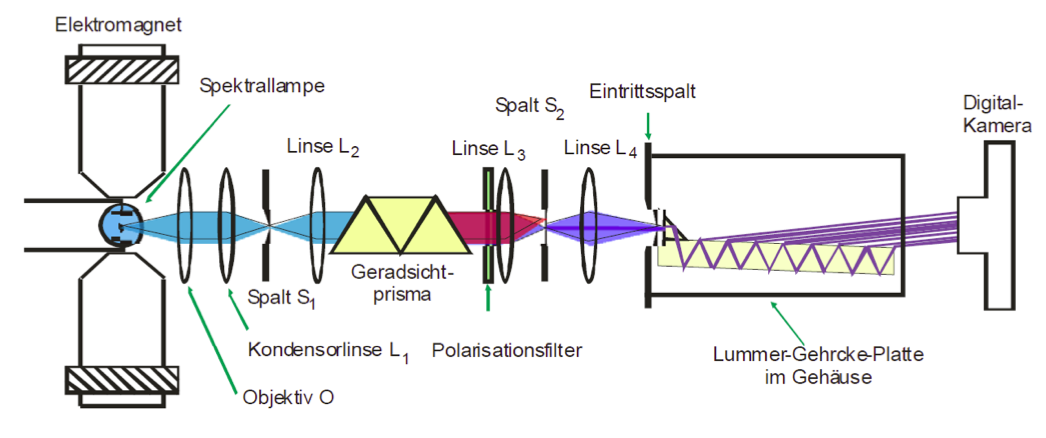
\includegraphics[width=0.8\textwidth]{images/Aufbau.png}
%    \caption{Schematische Darstellung des verwendeteten Versuchsaufbau zur Untersuchung der Zeeman-Effektes \cite{anleitung}.}
%    \label{fig:aufbau}
%\end{figure} \noindent
Wie in der Abbildung zu erkennen ist befindet sich im Zentrum eines Elektromagneten die Spektrallampe. Das Licht
wird duch eine Linse auf einen größenverstellbaren Spalt fokussiert. Daraufhin passiert das Licht eine
weitere Linse bevor es durch ein Geradsichtprisma in seine spektralen Anteile aufgespalten wird.
Mithilfe einer Kombination aus Linsen und einem weiteren Spalt wird die zu untersuchende Wellenlänge
auf den Eintrittsspalt der Lummer-Gehrcke-Platte gelenkt. Im Inneren dieser befinden sich parallele Platten
an denen das Licht reflektiert wird, wobei immer ein geringer Anteil aus dem Glas austritt.
Dadurch kommt es zu Interferenzerscheinungen, die mithilfe einer Digitalkamera aufgenommen werden.\\
Es ist sicherzustellen, dass die optischen Bauteile so eingestellt sind, dass eine möglichst hohe
Intensität in die Lummer-Gehrcke-Platte einfällt. \\
Im ersten Schritt der Messungen wird das Magnetfeld geeicht. Dafür wird das Magnetfeld im Inneren
des Elektromagneten mithilfe einer Hallsonde in Abhängigkeit des angelegten Stroms vermessen.
Daraufhin wird die rote Spektrallinie bei einer Magnetfeldstärke von ca. $\SI{650}{\milli\tesla}$ bei zwei
unterschiedlichen Einstellung des Polarisationsfilters untersucht. Analog wird für die blaue
Spektrallinie vorgegangen. Für die $\pi$-Linie wird ein Magnetfeld von ca. $\SI{280}{\milli\tesla}$
und für die $\sigma$-Linie eines von ca. $\SI{1120}{\milli\tesla}$ verwendet.
